% Section 2 - Behavior trees
% Roberto Masocco <roberto.masocco@uniroma2.it>
% May 24, 2026

% ### Behavior trees ###
\section{Behavior trees}
\graphicspath{{figs/section2/}}

% --- From states to trees ---
\begin{frame}{From states to trees}
  \justifying
  We now turn to a different formalism, \textbg{born in game AI} and now \textbg{ubiquitous in robotics}: the \textbg{behavior tree} (BT).\\
  \bigskip
  Behavior trees are
  \begin{itemize}
    \item \textbg{naturally active}: an execution model is built into the formalism;
    \item \textbg{modular}: each subtree is a complete behavior, composable with others;
    \item \textbg{reactive by construction}: the tree is re-evaluated at every step.
  \end{itemize}
  \bigskip
  The \textbg{reference implementation} is the C++ library \href{https://www.behaviortree.dev}{\color{blue}\underline{\texttt{BehaviorTree.CPP}}}.
\end{frame}

% --- Behavior trees ---
\begin{frame}{Behavior trees}{What is a BT?}
  \justifying
  A behavior tree is a \textbg{directed rooted tree} whose \textbg{nodes encode the logic} of a mission.\\
  \bigskip
  Two families of nodes exist:
  \begin{itemize}
    \item \textbg{internal nodes} (\textbg{control nodes}, \textbg{decorators}) compose the behavior of their children;
    \item \textbg{leaf nodes} (\textbg{actions}, \textbg{conditions}) interface with the rest of the system.
  \end{itemize}
  \bigskip
  \begin{block}{}
    \centering
    The \textbf{tree} is the \textbf{program}; \textbf{ticking} it is the \textbf{execution}.
  \end{block}
\end{frame}
\begin{frame}{Behavior trees}{Anatomy of a tree}
  \begin{figure}
    \centering
    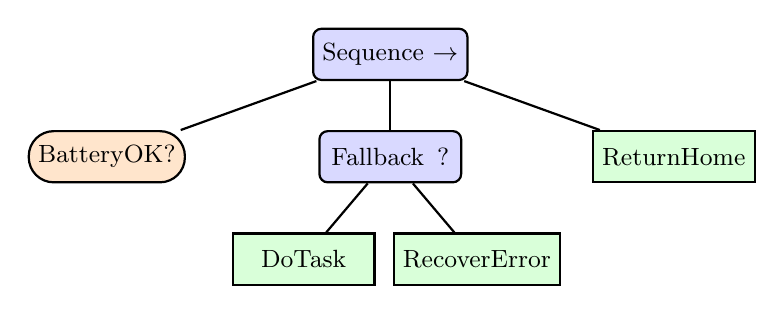
\begin{tikzpicture}[
      level distance=1.3cm,
      level 1/.style={sibling distance=3.6cm},
      level 2/.style={sibling distance=2.2cm},
      every node/.style={font=\small},
      ctrl/.style={draw, rounded corners=3pt, fill=blue!15, minimum width=1.8cm, minimum height=0.65cm, thick},
      act/.style={draw, fill=green!15, minimum width=1.8cm, minimum height=0.65cm, thick},
      cond/.style={draw, rounded corners=9pt, fill=orange!20, minimum width=1.8cm, minimum height=0.65cm, thick},
      edge from parent/.style={draw, thick}
    ]
      \node[ctrl] {Sequence $\rightarrow$}
        child {node[cond] {BatteryOK?}}
        child {node[ctrl] {Fallback \,?}
          child {node[act] {DoTask}}
          child {node[act] {RecoverError}}
        }
        child {node[act] {ReturnHome}};
    \end{tikzpicture}
    \caption{A small behavior tree, with a \texttt{Sequence} root, a nested \texttt{Fallback} subtree, an action ($\square$), a condition ($\ovalbox{\phantom{}}$) and a recovery alternative.}
  \end{figure}
\end{frame}
\begin{frame}{Behavior trees}{Ticks and execution order}
  \justifying
  Execution is driven by \textbg{ticks}: a \textbg{periodic signal} sent from the \textbg{root} of the tree.\\
  \bigskip
  When ticked, an internal node \textbg{forwards the tick} to its children according to its own policy.
  \begin{block}{}
    \centering
    \textbf{The traversal is always top to bottom, left to right.}
  \end{block}
  \bigskip
  The \textbg{order of children} therefore matters: it encodes \textbg{priority}. A tree is \textbg{single-threaded at the tick level} --- the root sees a sequence of ticks, never a parallel one.
\end{frame}
\begin{frame}{Behavior trees}{Return statuses}
  \justifying
  Every node, when ticked, \textbg{returns} one of three statuses:
  \begin{itemize}
    \item \texttt{SUCCESS}: the node has completed its task successfully;
    \item \texttt{FAILURE}: the node has failed;
    \item \texttt{RUNNING}: the node is in progress, and needs more ticks.
  \end{itemize}
  \bigskip
  \begin{block}{The three-status calculus}
    \justifying
    The \textbf{return value flows up} the tree from the ticked node to the root: each control node interprets the statuses of its children and computes its own status from them.
  \end{block}
\end{frame}
\begin{frame}{Behavior trees}{Leaves}
  \justifying
  Leaves are where the tree meets the rest of the system.
  \begin{itemize}
    \item \textbg{Action nodes}: do actual work --- move the robot, call a service, run a computation. They \textbg{may be asynchronous}, and can return \texttt{RUNNING} until completion.
    \item \textbg{Condition nodes}: evaluate a predicate --- is the battery full? is the target visible? They are \textbg{synchronous} and can only return \texttt{SUCCESS} or \texttt{FAILURE}.
  \end{itemize}
  \bigskip
  \begin{block}{}
    \centering
    \textbf{Conditions never block; actions may.}
  \end{block}
\end{frame}

% --- Control nodes ---
\begin{frame}{Control nodes}{Overview}
  \justifying
  \texttt{BT.CPP} provides three main families of \textbg{nodes that control the execution flow}:
  \begin{itemize}
    \item \textbg{Sequence}: run children one after the other, all must succeed (AND);
    \item \textbg{Fallback} (or \textbg{Selector}): try children in order, at least one must succeed (OR);
    \item \textbg{Parallel}: tick all children in the same cycle.
  \end{itemize}
  \bigskip
  Each family has \textbg{plain} and \textbg{reactive} variants, with subtly different semantics.
\end{frame}
\begin{frame}{Control nodes}{Sequence and Fallback}
  \justifying
  Plain \textbg{Sequence} (\texttt{$\rightarrow$}):
  \begin{itemize}
    \item ticks children left-to-right;
    \item returns \texttt{FAILURE} on the first \texttt{FAILURE}, \texttt{RUNNING} if a child is \texttt{RUNNING}, \texttt{SUCCESS} if all children succeed.
  \end{itemize}
  \bigskip
  Plain \textbg{Fallback} (\texttt{?}):
  \begin{itemize}
    \item ticks children left-to-right;
    \item returns \texttt{SUCCESS} on the first \texttt{SUCCESS}, \texttt{RUNNING} if a child is \texttt{RUNNING}, \texttt{FAILURE} if all children fail.
  \end{itemize}
  \bigskip
  \begin{block}{Memory of plain controls}
    \justifying
    On a re-tick after \texttt{RUNNING}, \textbf{plain controls resume from the running child}, skipping the children that have already completed.
  \end{block}
\end{frame}
\begin{frame}{Control nodes}{Two examples}
  \begin{figure}
    \centering
    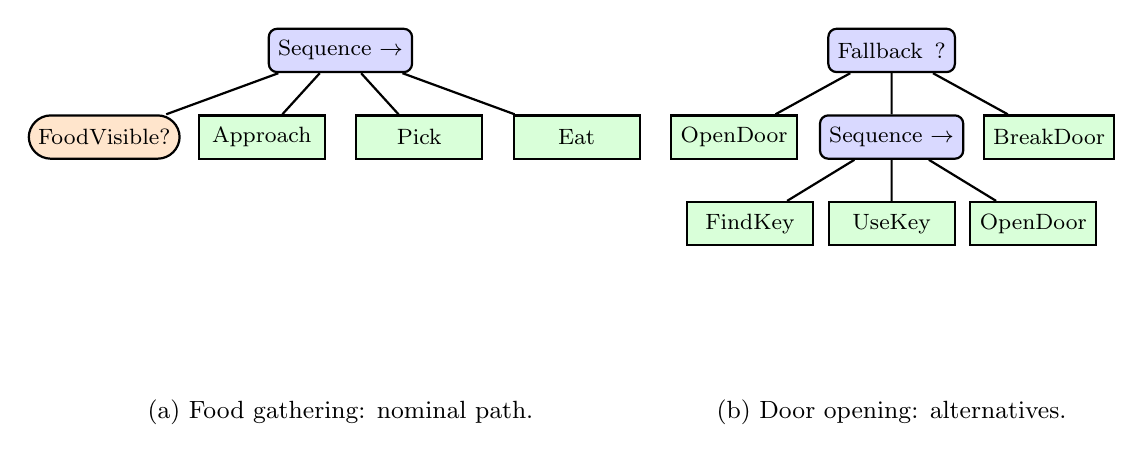
\begin{tikzpicture}[
      level distance=1.1cm,
      level 1/.style={sibling distance=2cm},
      level 2/.style={sibling distance=1.8cm},
      every node/.style={font=\footnotesize},
      ctrl/.style={draw, rounded corners=3pt, fill=blue!15, minimum width=1.6cm, minimum height=0.55cm, thick},
      act/.style={draw, fill=green!15, minimum width=1.6cm, minimum height=0.55cm, thick},
      cond/.style={draw, rounded corners=8pt, fill=orange!20, minimum width=1.6cm, minimum height=0.55cm, thick},
      edge from parent/.style={draw, thick}
    ]
      \node[ctrl] (root) at (0,0) {Sequence $\rightarrow$}
        child {node[cond] {FoodVisible?}}
        child {node[act] {Approach}}
        child {node[act] {Pick}}
        child {node[act] {Eat}};
      \node[font=\small] at (0,-4.6) {(a) Food gathering: nominal path.};

      \begin{scope}[xshift=7.0cm]
        \node[ctrl] (root2) at (0,0) {Fallback \,?}
          child {node[act] {OpenDoor}}
          child {node[ctrl] {Sequence $\rightarrow$}
            child {node[act] {FindKey}}
            child {node[act] {UseKey}}
            child {node[act] {OpenDoor}}
          }
          child {node[act] {BreakDoor}};
        \node[font=\small] at (0,-4.6) {(b) Door opening: alternatives.};
      \end{scope}
    \end{tikzpicture}
    \caption{Two canonical patterns: \texttt{Sequence}-based happy path (a) and \texttt{Fallback}-based recovery cascade (b).}
  \end{figure}
\end{frame}
\begin{frame}{Control nodes}{Reactive variants}
  \justifying
  \textbg{ReactiveSequence} and \textbg{ReactiveFallback} differ from their plain siblings on one point: on a re-tick, they do not skip the already-completed children.\\
  They \textbg{re-tick every child from the first one, every tick}.\\
  \bigskip
  This is essential when \textbg{preconditions can change during execution}: a condition that succeeded one tick ago may have flipped, and a reactive control will catch it; a plain one will not.\\
  \bigskip
  \begin{alertblock}{Plain vs reactive}
    \justifying
    \textbr{Plain} controls have \textbr{memory} of past successes: they are appropriate when ``done is done''. \textbr{Reactive} controls re-evaluate everything every tick: they are appropriate when the world keeps changing.
  \end{alertblock}
\end{frame}
\begin{frame}{Control nodes}{Parallel and ParallelAll}
  \justifying
  The \textbg{Parallel} family ticks \textbg{all children in the same cycle}, then \textbg{aggregates} their statuses.\\
  \bigskip
  \textbg{Parallel} uses \textbg{thresholds}:
  \begin{itemize}
    \item returns \texttt{SUCCESS} as soon as a \textbg{configurable number} of children \textbg{succeed};
    \item returns \texttt{FAILURE} as soon as a \textbg{configurable number} of children \textbg{fail}.
  \end{itemize}
  \bigskip
  \textbg{ParallelAll} is stricter: it \textbg{waits for every child to complete} before deciding. No early exit.\\
  \bigskip
  Both are the right tool when \textbg{several independent behaviors must progress together} --- for example, navigate while keeping an eye on the battery and on a target detector.
\end{frame}
\begin{frame}{Control nodes}{Concurrency, not parallelism}
  \justifying
  \textbg{Parallel} does \textbg{not} mean ``parallel threads''. The tree is single-threaded: within one tick cycle, a \texttt{Parallel} node ticks its children \textbg{one after another, in order}.\\
  \bigskip
  What enables apparent simultaneity is the fact that \textbg{action leaves can be asynchronous}: an action returns \texttt{RUNNING} immediately, while the underlying computation \textbg{keeps progressing between ticks}.\\
  \bigskip
  \begin{alertblock}{The right mental model}
    \justifying
    \textbr{Concurrent progress} of long-running actions, \textbr{sequential traversal} of the tree.\\
    \textbr{Long blocking work belongs in an asynchronous action}, never inside the tick of a synchronous one.
  \end{alertblock}
\end{frame}

% --- Decorators and the blackboard ---
\begin{frame}{Decorators}
  \justifying
  A \textbg{decorator} is an internal node with \textbg{exactly one child}: it modifies the child's behavior in some way.\\
  \bigskip
  The most common decorators in BT.CPP:
  \begin{itemize}
    \item \textbg{Inverter}: swaps \texttt{SUCCESS} and \texttt{FAILURE};
    \item \textbg{Retry}: re-ticks the child up to $N$ times on \texttt{FAILURE};
    \item \textbg{Repeat}: re-ticks the child up to $N$ times on \texttt{SUCCESS};
    \item \textbg{Timeout}: fails the child if it does not finish within a time budget;
    \item \textbg{ForceSuccess}, \textbg{ForceFailure}: ignore the child's status and return a fixed one.
  \end{itemize}
  \bigskip
  Decorators turn primitives into reusable, parameterized behaviors.
\end{frame}
\begin{frame}{The blackboard}
  \justifying
  Nodes need to \textbg{exchange data}: the result of a detection action must reach the navigation action, a parameter must reach the right leaf, and so on.\\
  \bigskip
  \texttt{BT.CPP} solves this with the \textbg{blackboard}: a \textbg{typed, shared key-value store accessible to all nodes} in the tree.\\
  \bigskip
  Nodes declare \textbg{ports}:
  \begin{itemize}
    \item \textbg{input ports}: read from the blackboard;
    \item \textbg{output ports}: write to the blackboard.
  \end{itemize}
  Ports can be \textbg{wired} as in, \emph{e.g.}, a Simulink diagram, to implement a flow of information across ticks.
\end{frame}

% --- BehaviorTree.CPP ---
\begin{frame}[fragile]{BehaviorTree.CPP}{The tree XML}
  \justifying
  \texttt{BT.CPP} loads trees from \textbg{XML files}: the structure of the tree is data, separate from the implementation of its nodes. A \href{https://www.behaviortree.dev/docs/tutorial-basics/tutorial_09_scripting/}{\color{blue}\underline{\textbf{scripting language}}} can be used to perform operations on variables in the XML.
  \begin{columns}
    \column{.9\textwidth}
    \begin{lstlisting}[language=btcppxml, caption=Example XML file for the food-gathering tree; the first three leaf nodes have ports; they are all wired together pointing the same blackboard entry \texttt{food\_pose} (curly braces).]
<root BTCPP_format="4">
  <BehaviorTree ID="GatherFood">
    <Sequence name="root">
      <FoodVisible target="{food_pose}"/>
      <Approach    goal="{food_pose}"/>
      <Pick        target="{food_pose}"/>
      <Eat/>
    </Sequence>
  </BehaviorTree>
</root>
\end{lstlisting}
  \end{columns}
\end{frame}
\begin{frame}[fragile]{BehaviorTree.CPP}{Custom node classes}
  \justifying
  \textbg{Each node is a C++ class inheriting from a base provided by the library.}\\
  \bigskip
  \only<1>{
    There are \textbg{four relevant categories}:
    \begin{itemize}
      \item \textbg{actions};
      \item \textbg{conditions};
      \item \textbg{controls};
      \item \textbg{decorators}.
    \end{itemize}
  }
  \only<2>{
    \textbg{Actions} may be of multiple \textbg{types}.
    \begin{description}
      \item[\texttt{SyncActionNode}] has only a \texttt{tick()} method, which must return either \texttt{SUCCESS} or \texttt{FAILURE}.
      \item[\texttt{StatefulActionNode}] may return \texttt{RUNNING} for prolonged operations and be \textbg{interrupted}.
        \begin{itemize}
          \item \texttt{onStart()} method must gather data and \textbg{start the operation}, returning \texttt{RUNNING} if all is good;
          \item \texttt{onRunning()} method \textbg{does the job} and may return any of the three states;
          \item \texttt{onHalted()} is invoked \textbg{when the operation must stop} to clean up, as in \textbg{preemption}.
        \end{itemize}
      \item[\texttt{CoroActionNode}] may be used to implement actions that can be \textbg{paused}.
    \end{description}
  }
  \only<3>{
    \textbg{Conditions} inherit from \texttt{ConditionNode}.\\
    \bigskip
    They are \textbg{leaves that may only do a quick check} in their \texttt{tick()} method, returning either \texttt{SUCCESS} or \texttt{FAILURE}.\\
    \bigskip
    Almost everything can be done with a \texttt{ScriptCondition} node.
  }
  \only<4>{
    \textbg{Controls} inherit from \texttt{ControlNode}. They
    \begin{itemize}
      \item may have \textbg{multiple children};
      \item implement a \textbg{policy} to decide if, when, and how many children get ticked afterwards.
    \end{itemize}
    \bigskip
    The library offers many Controls which implement many \textbg{common control flow constructs}, it is unlikely that you may need to add more.
  }
  \only<5>{
    \textbg{Decorators} inherit from \texttt{DecoratorNode}. They
    \begin{itemize}
      \item have \textbg{only a single child};
      \item may \textbg{alter} the result of their child;
      \item may \textbg{control when or how many times} their child is ticked;
      \item may tick their child imposing \textbg{conditions or constraints}.
    \end{itemize}
    \bigskip
    The library offers many Decorators which implement many \textbg{unary operators}, it is unlikely that you may need to add more.
  }
\end{frame}

% --- dua_behaviortree_cpp ---
\begin{frame}{\texttt{dua\_behaviortree\_cpp}}{Behavior Trees meet ROS~2}
  \justifying
  The \href{https://github.com/dotX-Automation/dua_behaviortree_cpp}{\color{blue}\underline{\texttt{dua\_behaviortree\_cpp}}} repository integrates \texttt{BT.CPP} with ROS~2.\\
  \bigskip
  It houses \textbg{four packages}:
  \begin{itemize}
    \item \texttt{btcpp\_executor}: \textbg{composable node} acting as the \textbg{BT executor};
    \item \texttt{dua\_btcpp\_base}: \textbg{base class} for custom BT.CPP node extensions, built on \href{https://docs.ros.org/en/jazzy/Tutorials/Beginner-Client-Libraries/Pluginlib.html}{\color{blue}\underline{\texttt{pluginlib}}};
    \item \texttt{dua\_btcpp\_types}: \textbg{custom data types} for the integration;
    \item \texttt{dua\_btcpp\_nodes}: a \textbg{library of ready-made nodes} for common use cases (everyday actions, services, etc.).
  \end{itemize}
  \bigskip
  You may \textbg{implement your node library} by \textbg{inheriting from the register class} in \texttt{dua\_btcpp\_base}.
\end{frame}
\begin{frame}{\texttt{dua\_behaviortree\_cpp}}{Runtime model}
  The \texttt{dua\_behaviortree\_cpp} framework is \textbg{designed for continously-running BTs}.\\
  \bigskip
  Thus, in \texttt{dua\_btcpp\_nodes} and \texttt{btcpp\_executor} especially, the following \textbg{convention on node return states} is adopted.
  \begin{description}
    \item[\texttt{RUNNING}] is returned when all is well, and propagated to the root to signal that \textbg{the tree is still being executed}.
    \item[\texttt{SUCCESS}] shall be returned by instantaneous checks and conditions or by actions, but \textbg{only propagated to the root when the tree has to stop successfully}.
    \item[\texttt{FAILURE}] shall be returned \textbg{on any unrecoverable error} and \textbg{immediately propagated to the root}.
  \end{description}
\end{frame}
\begin{frame}{\texttt{dua\_behaviortree\_cpp}}{Runtime model}
  \justifying
  At startup, the \texttt{btcpp\_executor}:
  \begin{enumerate}
    \item \textbg{reads its parameters}: tree XML path, list of BT node \textbg{plugin libraries} to load;
    \item \textbg{loads each plugin library} through \texttt{pluginlib}, registering every node it exposes into the BT.CPP factory;
    \item parses the XML and \textbg{instantiates the tree};
    \item starts \textbg{ticking}.
  \end{enumerate}
  \bigskip
  \begin{block}{Composable node}
    \justifying
    Being a \textbf{composable node}, the executor can be loaded into the same process as other ROS 2 nodes, sharing intra-process communications and reducing latency for the action and service calls issued by the BT leaves.
  \end{block}
\end{frame}

% --- The executor pattern ---
\begin{frame}{The executor pattern}{\texttt{transitions\_ros} vs \texttt{dua\_behaviortree\_cpp}}
  \justifying
  The same architectural idea appears in both formalisms.
  \begin{columns}[T]
    \column{.48\textwidth}
    \begin{block}{\texttt{transitions\_ros}}
      \justifying
      A generic \textbf{\texttt{machine\_executor}} node loads, at runtime, a Python module containing:
      \begin{itemize}
        \item a transitions table;
        \item a states table with per-state routines.
      \end{itemize}
      \textbf{The mission lives in the module, not in the executor.}
    \end{block}
    \column{.48\textwidth}
    \begin{block}{\texttt{dua\_behaviortree\_cpp}}
      \justifying
      A generic \textbf{\texttt{btcpp\_executor}} node loads, at runtime:
      \begin{itemize}
        \item a tree XML;
        \item one or more node plugin libraries.
      \end{itemize}
      \textbf{The mission lives in the XML and the plugins, not in the executor.}
    \end{block}
  \end{columns}
  \bigskip
  \begin{block}{}
    \centering
    Same pattern, two formalisms: generic executor, runtime-loaded domain logic.
  \end{block}
\end{frame}

% --- Use case: Leonardo Drone Contest ---
\begin{frame}{Use case: Leonardo Drone Contest}{Overview}
  % TODO: contest, year, what changed from last year's mission.
\end{frame}
\begin{frame}{Use case: Leonardo Drone Contest}{Why the FSM exploded}
  % TODO: concrete reasons the FSM approach broke down (states count, reactive conditions, recovery branches).
\end{frame}
\begin{frame}{Use case: Leonardo Drone Contest}{BT diagram}
  % TODO: insert the BT diagram image of the contest mission here.
  \begin{center}
    \textit{[Behavior tree of the contest mission.]}
  \end{center}
\end{frame}
\begin{frame}{Use case: Leonardo Drone Contest}{Design decisions}
  % TODO: reactive vs plain controls, where Parallel was used, blackboard layout.
\end{frame}
\begin{frame}{Use case: Leonardo Drone Contest}{Results}
  % TODO: what worked, comparison with the FSM-era effort.
\end{frame}

% --- Wrap-up ---
\begin{frame}{Wrap-up}
  \justifying
  Takeaways from this section:
  \begin{itemize}
    \item \textbg{behavior trees} replace ``one state at a time'' with ``one tree, ticked'';
    \item \textbg{control nodes} (Sequence, Fallback, Parallel, with their reactive variants) provide the calculus, \textbg{leaves} provide the substance, \textbg{decorators} the connective tissue;
    \item \href{https://github.com/BehaviorTree/BehaviorTree.CPP}{\color{blue}\underline{\texttt{BehaviorTree.CPP}}} is the de-facto C++ library; \href{https://github.com/dotX-Automation/dua_behaviortree_cpp}{\color{blue}\underline{\texttt{dua\_behaviortree\_cpp}}} integrates it as a ROS~2 composable executor with \texttt{pluginlib}-loaded nodes;
    \item the same \textbg{executor pattern} we already saw in \texttt{transitions\_ros} reappears: a generic engine, domain logic loaded at runtime.
  \end{itemize}
\end{frame}
